\chapter{Aportaciones}

\section{Redes Neuronales Totalmente Conectadas}

\subsection{Gradiente de la función de pérdida respecto a SoftMax, \cite{Cross_entropy_backprop} \cite{Cross_entropy_backprop_grad_input}} 

Siendo $Z_i$ la entrada $i$ de la última capa, se denotará mediante $O_i$ una vez se le aplique SoftMax. \\

\begin{figure}[H]
	\centering
	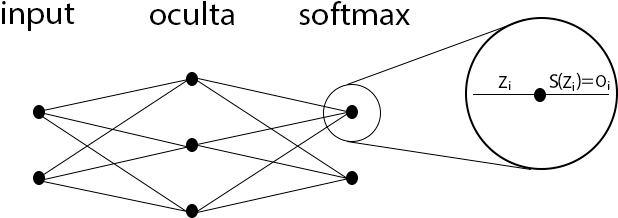
\includegraphics[scale=0.4]{imagenes/NN_softmax.jpg}  
	\caption{Estructura de una red con softmax}
\end{figure}

\begin{gather}
	E = - \sum_{i=1}^{H}  [y_i * log(O_i)] 
	\label{cross_entropy_notacion}
\end{gather}

Según esta notación, la función de error \ref{loss_func_softmax} se convierte en la fórmula \ref{cross_entropy_notacion}.

\subsubsection{Gradiente de la función de error}

\begin{gather}
	\frac{\partial E}{\partial Z_k} = \frac{\partial(- \sum_{i=1}^{H}  [y_i * log(O_i)])}{\partial Z_k} = - \sum_{i=1}^{H}  [\frac{\partial(y_i * log(O_i))}{\partial Z_k}] 
\end{gather}

Como $y_i$ es independiente respecto a $Z_k$, se trata como una constante. \\
\begin{gather}
	\frac{\partial E}{\partial Z_k} = - \sum_{i=1}^{H}  [y_i * \frac{\partial(log(O_i))}{\partial Z_k}] 
\end{gather}

Se aplica la regla de la cadena, pues $O_i$ no depende directamente de $Z_k$,. \\
\begin{gather}	
	\frac{\partial E}{\partial Z_k} = - \sum_{i=1}^{H}  [y_i * \frac{\partial(log(O_i))}{\partial O_i} * \frac{\partial O_i}{\partial Z_k}] \\
	\frac{\partial E}{\partial Z_k} = - \sum_{i=1}^{H}  [\frac{y_i}{O_i} * \frac{\partial O_i}{\partial Z_k}] 
	\label{gradiente_Oi_Zk}
\end{gather}

% ver https://www.mldawn.com/the-derivative-of-softmaxz-function-w-r-t-z/

\subsubsection{Derivada de softmax respecto de su entrada, $\frac{\partial O_i}{\partial Z_k}$}

Hay 2 casos posibles, $\frac{S(Z_i)}{Z_i}$ o $\frac{S(Z_i)}{Z_j}$, donde i $\neq$ j. \\

\subsubsection{Caso $\frac{S(Z_i)}{Z_i}$}

\begin{gather}
	\frac{\partial f(x)}{\partial g(x)} = \frac{f'(x)*g(x) - g'(x)*f(x)}{g(x)^2} \\
	S(z_i) = \frac{e^{Z_i}}{e^{Z_1} + ... + e^{Z_H}} \\
	\frac{\partial S(Z_1)}{\partial Z_1} = \frac{[\frac{\partial e^{Z_1}}{\partial Z_1} * (e^{Z_1} + ... + e^{Z_H}) ] - [\frac{\partial (e^{Z_1} + ... + e^{Z_H})}{\partial Z_1} * e^{Z_1} ] }{(e^{Z_1} + ... + e^{Z_H})^2} 
\end{gather}

Se aplica $\frac{\partial e^{Z_1}}{Z_1} = e^{Z_1}$ \\
\begin{gather}
	\frac{\partial S(Z_1)}{\partial Z_1} = \frac{[e^{Z_1} * \sum_{i=1}^{H}  e^{Z_i}] - [e^{Z_1} * e^{Z_1}]   }{ (\sum_{i=1}^{H}  e^{Z_i})^2} \\
\end{gather}

Se saca factor común $e^{Z_1}$ \\
\begin{gather}
	\frac{\partial S(Z_1)}{\partial Z_1} = \frac{e^{Z_1} ([\sum_{i=1}^{H}  e^{Z_i}] - e^{Z_1})  }{(\sum_{i=1}^{H}  e^{Z_i})^2} \\
	\frac{\partial S(Z_1)}{\partial Z_1} = \frac{e^{Z_1}}{\sum_{i=1}^{H}  e^{Z_i}} * \frac{[\sum_{i=1}^{H}  e^{Z_i}] - e^{Z_1}}{\sum_{i=1}^{H}  e^{Z_i}}
\end{gather}

Se recuerda que $\frac{\sum_{i=1}^{H}  e^{Z_i}}{\sum_{i=1}^{H}  e^{Z_i}} = 1$ y que S($Z_1$) = $ \frac{e^{Z_1}}{\sum_{i=1}^{H}  e^{Z_i}}$ \\
\begin{gather}
	\frac{\partial S(Z_1)}{\partial Z_1} = S(Z_1) * (1- S(Z_1))
	\label{grad_Oi_Zk_drch}
\end{gather}

\subsubsection{Caso $\frac{S(Z_i)}{Z_j}$, con i $\neq$ j}

\begin{gather}
	\frac{\partial S(Z_2)}{\partial Z_1} = \frac{[\frac{\partial e^{Z_2}}{\partial Z_1} * (e^{Z_1} + ... + e^{Z_H}) ] - [\frac{\partial (e^{Z_1} + ... + e^{Z_H})}{\partial Z_1} * e^{Z_2} ] }{(e^{Z_1} + ... + e^{Z_H})^2} \\
	\frac{\partial S(Z_2)}{\partial Z_1} = \frac{[0 * [\sum_{i=1}^{H}  e^{Z_i}]] - [e^{Z_1} * e^{Z_2}]   }{ (\sum_{i=1}^{H}  e^{Z_i})^2} \\
	\frac{\partial S(Z_2)}{\partial Z_1} = \frac{-e^{Z_1} * e^{Z_2}  }{(\sum_{i=1}^{H}  e^{Z_i})^2} \\
	\frac{\partial S(Z_2)}{\partial Z_1} = \frac{-e^{Z_1}}{\sum_{i=1}^{H}  e^{Z_i}} * \frac{e^{Z_2}}{\sum_{i=1}^{H}  e^{Z_i}} \\
	\frac{\partial S(Z_2)}{\partial Z_1} = -S(Z_1) * S(Z_2)
	\label{grad_Oi_Zk_izq}
\end{gather}

\subsubsection{Combinación de casos}

De esta forma, tendremos que dividir  el proceso en 2 partes, cuando i sea igual a j, y cuando i $\neq$ j, perteneciendo a la primera todos los casos menos uno. \\
Parte izquierda cuando i!=k, parte derecha cuando i=k. \\
Retomamos la fórmula \ref{gradiente_Oi_Zk}, aplicando \ref{grad_Oi_Zk_izq} en la parte izquierda y \ref{grad_Oi_Zk_drch} en la derecha. \\
\begin{gather}
	\frac{\partial E}{\partial Z_k} = - [\sum_{i!=k}^{H} [\frac{y_i}{O_i} * -O_i * O_k ] + \frac{y_k}{O_k} * O_k * (1 - O_k)  ]
\end{gather}

Se simplifica $O_i$ en la parte izquierda y $O_k$ en la derecha. \\
\begin{gather}
	\frac{\partial E}{\partial Z_k} = - [\sum_{i!=k}^{H} [- y_i * O_k] + [y_k * (1 - O_k) ] ] 
\end{gather}

Se extrae $O_k$ de la suma, pues es independiente respecto al índice $i$ \\
\begin{gather}	
	\frac{\partial E}{\partial Z_k} = - [-O_k \sum_{i!=k}^{H}- y_i + [y_k * (1 - O_k) ] ]
	\label{simplificar}
\end{gather}

\subsubsection{Simplificación One-Hot}

Al emplear la codificación one-hot en Y, se sabe que la suma de sus elementos es igual a 1. \\
\begin{gather}
	\sum_{i=1}^{H} y_i = 1 \\
	\sum_{i!=k}^{H} y_i = \sum_{i=1}^{H} y_i - y_k = 1 - y_k
	\label{one_hot_simplif}
\end{gather}

Se emplea \ref{one_hot_simplif} para simplificar la suma en \ref{simplificar}. \\


\begin{gather}
	\frac{\partial E}{\partial Z_k} = [O_k*(1-y_k)] - [y_k*(1-O_k)] \\
	\frac{\partial E}{\partial Z_k} = O_k - O_k * y_k - y_k + O_k * y_k 
\end{gather}

Se simplifica $O_k*y_k$. \\
\begin{gather}
	\frac{\partial E}{\partial Z_k} = O_k - y_k = gradiente\_Z_k
	\label{gradiente_softmax}
\end{gather}

\subsection{BackPropagation con 1 capa oculta \cite{NN_backpropagation} \cite{NN_backprop_2} \label{backprop_1_capa}}

\begin{figure}[H]
	\centering
	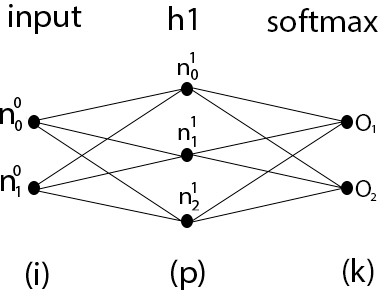
\includegraphics[scale=0.35]{imagenes/nn_1_capa.jpg}  
	\caption{Red Neuronal totalmente conectada con 1 capa oculta}
	\label{fig:nn_1_capa}
\end{figure}

La Figura \ref{fig:nn_1_capa} se compone de 'puntos' interconectados mediante líneas, representando neuronas y pesos que las conectan respectivamente. Cada punto corresponde a una neurona, y cada línea a un peso. \\
La Figura \ref{fig:nn_1_capa} presenta 3 capas (input, h1, softmax) que corresponden a capa de entrada, capa oculta $h_1$, y capa de salida respectivamente. El superíndice indica la capa a la que pertenece una neurona o peso, mientras que el subíndice indica el número del mismo en su respectiva capa. En el caso de los pesos, se requieren 2 subíndices para identificar a cada uno (pues un peso une 2 neuronas). \\
La capa de entrada se compone de 2 neuronas ($n^{0}_0$ y $n^{0}_1$). \\
La capa oculta $h_1$ tiene 3 neuronas ($n^1_{0}$, $n^1_{1}$, y $n^1_{2}$) \\
El peso $W^{i}_{jk}$ referencia al peso que une las neuronas $n^{i}_j$ y $n^{i+1}_k$.\\
De forma adicional, se recuerda que $Z_i$ representa la entrada $i$ de la capa SoftMax, y $O_i$ su salida.  

\subsubsection{Capa SoftMax}

\begin{figure}[H]
	\centering
	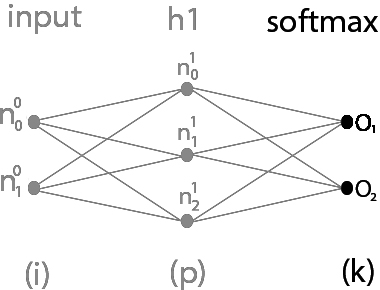
\includegraphics[scale=0.35]{imagenes/nn_1_capa_output.jpg}  
	\caption{Imagen de backpropagation en la capa softmax}
	\label{fig:nn_1_capa_output}
\end{figure}

Sea la neurona $n^i_j$, se define como $a^i_j$ el valor de dicha neurona antes de aplicar sobre ella su función de activación asociada, y $z^i_j$ el obtenido tras aplicarla. 

Tal y como se calculó previamente, el gradiente de la función de pérdida respecto a cada $Z_i$ viene dado por la fórmula \ref{gradiente_softmax}.


\subsubsection{Pesos capas h1-SoftMax}

\begin{figure}[H]
	\centering
	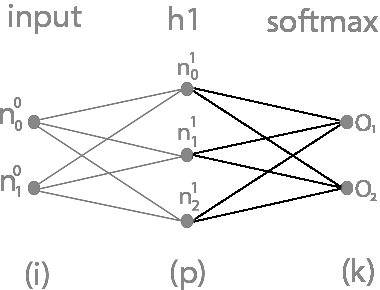
\includegraphics[scale=0.35]{imagenes/nn_1_capa_pesos_h1_output.jpg}  
	\caption{Imagen de backpropagation en los pesos entre la capa oculta y la capa SoftMax}
	\label{fig:nn_1_pesos_h1_output}
\end{figure}

Una vez calculado el gradiente hasta la capa softmax, se puede calcular el gradiente respecto a cada peso $W^1_{pk}$ que se encuentra conectado a esta desde la capa anterior. Es decir, para cada $h^1_p\in h_1$, se calcula $\frac{dE(x)}{dW^1_{pk}}$. Usando la regla de la cadena, equivale a realizar lo siguiente:


\begin{gather}
	\frac{\partial Z_k}{\partial W^1_{pk}} = \frac{\partial (z^1_p * W^1 _{pk}+ b^2_k)}{\partial W^1_{pk }} = z^1_p
	\label{grad_w1pk_1}
\end{gather}

\begin{gather}
	\frac{\partial E(x)}{\partial W^1_{pk }} =  gradiente\_Z_k * \frac{\partial Z_k}{\partial W^1_{pk }} = gradiente\_Z_k * z^1_p
	\label{grad_w1pk_2}
\end{gather}

\subsubsection{Sesgos capa softmax}

\begin{gather}
	\frac{\partial E}{\partial b^2_k} = \frac{\partial E}{\partial Z_k} * \frac{\partial Z_k}{b^2_k} \\
	\frac{\partial Z_k }{\partial b^2_k } = \frac{\partial ([\sum_{c=1}^{P} z^1_c * W^1_{pk}] + b^2_k) }{\partial b^2_k } = 1 \\
	\frac{\partial E}{\partial b^2_k} = gradiente\_Z_k
\end{gather}

\subsubsection{Capa oculta h1}

\begin{figure}[H]
	\centering
	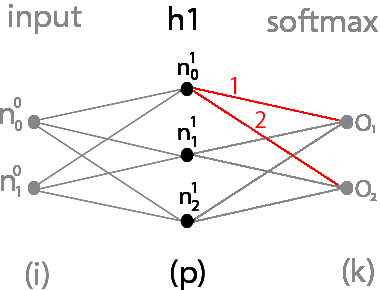
\includegraphics[scale=0.35]{imagenes/nn_caminos_posibles.jpg}  
	\caption{Imagen de los 'caminos' desde la capa softmax hasta $n^1_0$}
	\label{nn_caminos_posibles}
\end{figure}

En la figura \ref{nn_caminos_posibles} se muestra como hay más de un 'camino' desde la capa softmax hasta $n^1_p$. Por tanto, para obtener el gradiente de la pérdida respecto a $n^1_p$, habría que calcular la suma de todos los 'caminos' hacia este. \\

\begin{gather}
	\frac{\partial E_{total}}{\partial a^1_p} = \sum_{k=1}^K \frac{\partial E_k}{\partial a^1_p} = \sum_{k=1}^K  gradiente\_Z_k * \frac{\partial Z_k}{\partial z^1_p} * \frac{\partial z^1_p}{\partial a^1_p}
	\label{E_total_a1p}
\end{gather}

\begin{gather}
	\frac{\partial Z_k}{\partial z^1_p} = \frac{\partial( [\sum_{c=1}^{P} z^1_c * W^1_{ck}] + b^2_k)}{\partial z^1_p} = W^1_{pk}
	\label{deriv_Zk_z1p}
\end{gather}

\begin{figure}[H]
	\centering
	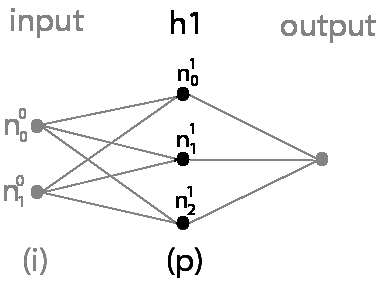
\includegraphics[scale=0.35]{imagenes/nn_1_capa_h1.jpg}  
	\caption{Imagen de backpropagation en la capa oculta h1}
	\label{fig:nn_1_capa_h1}
\end{figure}

En la capa oculta h1 se emplea la función de activación sigmoide. 

\begin{gather}
	sigmoide(x) = \frac{1}{1+e^{-x}} \\
	sigmoide'(x) = \frac{sigmoide(x)}{1-sigmoide(x)}
\end{gather}

De esta forma,

\begin{gather}
	\frac{\partial z^1_ p}{\partial a^1_p} = \frac{\partial sigmoide(a^1_p)}{\partial a^1_p} = sigmoide(a^1_p)*(1-sigmoide(a^1_p))
	\label{deriv_z1p_a1p}
\end{gather}

Se retoma la fórmula \ref{E_total_a1p} mediante la aplicación de \ref{deriv_Zk_z1p} y \ref{deriv_z1p_a1p}

\begin{gather}
	\frac{\partial E_{total}}{\partial a^1_p} = \sum_{k=1}^K  gradiente\_Z_k * W^1_{pk} * sigmoide(a^1_p)*(1-sigmoide(a^1_p)) \\
	\frac{\partial E_{total}}{\partial a^1_p} = gradiente\_h1_p
	\label{grad_E_a1p}
\end{gather}

\subsubsection{Pesos capas input-h1}

\begin{figure}[H]
	\centering
	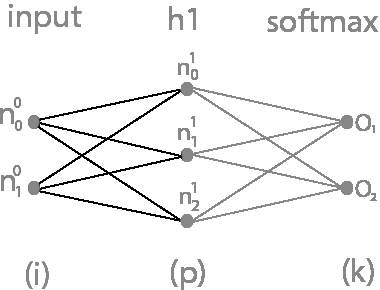
\includegraphics[scale=0.35]{imagenes/nn_1_capa_pesos_input_h1.jpg}  
	\caption{Imagen de backpropagation en los pesos entre la capa input y la capa oculta h1}
	\label{fig:nn_1_pesos_input_h1}
\end{figure}


\begin{gather}
	\frac{\partial a^1_p }{\partial W^0_{ip} } = \frac{\partial [\sum_{c=1}^{I} z^0_c * W^0_{cp}] + b^1_p)}{\partial W^0_{ip} } = z^0_i \\
	\frac{\partial E}{\partial W^0_{ip}} = \frac{\partial E_{total} }{\partial a^1_p } * \frac{\partial a^1_p}{W^0_{ip}} \\
	\frac{\partial E(x) }{\partial W^0_{ip} } = gradiente\_h1_p * \frac{\partial a^1_p }{\partial W^0_{ip} } = gradiente\_h1_p * z^0_i 
	\label{grad_w0ip}
\end{gather}

\subsubsection{Sesgos capa h1}

\begin{gather}
	\frac{\partial E}{\partial b^1_p} = \frac{\partial E_{total} }{\partial a^1_p } * \frac{\partial a^1_p}{b^1_p} \\
	\frac{\partial a^1_p }{\partial b^1_p } = \frac{\partial ([\sum_{c=1}^{I} z^0_c * W^0_{ip}] + b^1_p) }{\partial b^1_p } = 1 \\
	\frac{\partial E}{\partial b^1_p} = gradiente\_h1_p
	\label{grad_b1p}
\end{gather}

\subsubsection{Capa input}

\begin{figure}[H]
	\centering
	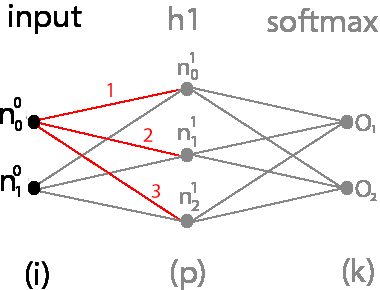
\includegraphics[scale=0.35]{imagenes/nn_caminos_posibles_input.jpg}  
	\caption{Imagen de los 'caminos' desde la capa oculta h1 hasta $n^0_0$}
	\label{nn_caminos_posibles_input}
\end{figure}

\begin{gather}
	\frac{\partial E_{total}}{\partial a^0_i} = \sum_{p=1}^P \frac{\partial E_{total}}{\partial a^1_p} * \frac{\partial a^1_p}{\partial z^0_i} * \frac{\partial z^0_i}{\partial a^0_i} \\
	\frac{\partial a^1_p }{\partial z^0_i } = \frac{\partial ([\sum_{c=1}^{I} z^0_c * W^0_{ip}] + b^1_p) }{\partial z^0_i } = W^0_{ip}
\end{gather}

\begin{figure}[H]
	\centering
	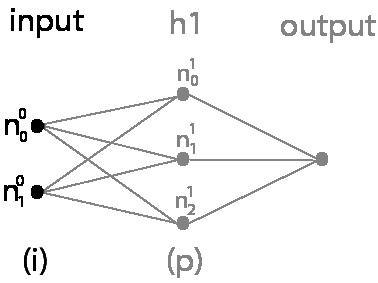
\includegraphics[scale=0.35]{imagenes/nn_1_capa_input.jpg}  
	\caption{Imagen de backpropagation en la capa input}
	\label{fig:nn_1_capa_input}
\end{figure}

Como la capa input no presenta ninguna función de activación asociada, $z^0_i$ es igual $a^0_i$. \\

\begin{gather}
	\frac{\partial z^0_i }{\partial a^0_i } = 1 \\
	\frac{\partial E_{total}}{\partial a^0_i} = \sum_{p=1}^{P} gradiente\_h1_p
\end{gather}

\subsection{Retropropagación con 2 capas ocultas}

\begin{figure}[H]
	\centering
	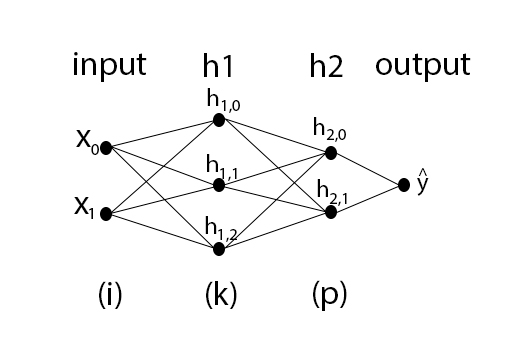
\includegraphics[scale=0.35]{imagenes/nn_2_capas.jpg}  
	\caption{Red Neuronal totalmente conectada con 2 capas ocultas}
	\label{fig:nn_2_capas}
\end{figure}

Tal y como muestra la Figura \ref{fig:nn_2_capas}, en este caso se emplea una red totalmente conectada con 2 capas ocultas (h1 y h2). \\

\subsubsection{Capa SoftMax}

\begin{figure}[H]
	\centering
	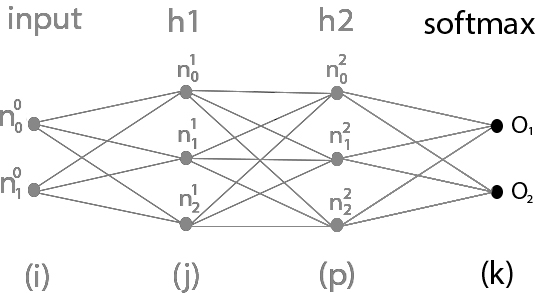
\includegraphics[scale=0.35]{imagenes/nn_2_capa_output.jpg}  
	\caption{Imagen de backpropagation en la capa softmax}
\end{figure}

Al igual que en el apartado anterior (\ref{backprop_1_capa}), el gradiente de la función de pérdida respecto a cada $Z_i$ viene dado por la fórmula \ref{gradiente_softmax}. \\

\subsubsection{Pesos capas h2-SoftMax}

\begin{figure}[H]
	\centering
	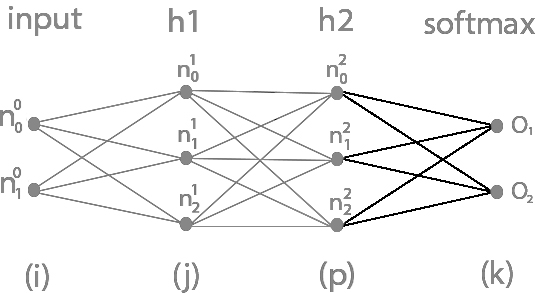
\includegraphics[scale=0.35]{imagenes/nn_2_capa_pesos_h2_output.jpg}  
	\caption{Imagen de backpropagation en los pesos entre la capa oculta h2 y la capa SoftMax}
\end{figure}

Se realiza el cálculo del gradiente de la función de pérdida respecto a cada peso $W^2_{pk}$ que une las neuronas de la capa oculta h2 con las de la capa de salida softmax. \\

\begin{gather}
	\frac{\partial Z_k}{\partial W^2_{pk}} = \frac{\partial (z^2_p * W^2 _{pk} + b^3_k)}{\partial W^2_{pk }} = z^2_p 
	\label{grad_w2pk_1}
\end{gather}

\begin{gather}
	\frac{\partial E(x)}{\partial W^2_{pk }} =  gradiente\_Z_k * \frac{\partial Z_k}{\partial W^2_{pk }} = gradiente\_Z_k * z^2_p
	\label{grad_w2pk_2}
\end{gather}

Como es de esperar, las fórmulas \ref{grad_w2pk_1} y \ref{grad_w2pk_2} son casi idénticas a \ref{grad_w1pk_1} y \ref{grad_w1pk_2} respectivamente, salvo por el superíndice empleado (1 $\neq$ 2). Esto tiene sentido pues esta parte también es común al apartado anterior.

\subsubsection{Sesgos capa softmax}

\begin{gather}
	\frac{\partial E}{\partial b^3_k} = \frac{\partial E}{\partial Z_k} * \frac{\partial Z_k}{b^3_k} \\
	\frac{\partial Z_k }{\partial b^3_k } = \frac{\partial ([\sum_{c=1}^{P} z^2_c * W^2_{pk}] + b^3_k) }{\partial b^3_k } = 1 \\
	\frac{\partial E}{\partial b^3_k} = gradiente\_Z_k
\end{gather}

\subsubsection{Capa oculta h2}

\begin{figure}[H]
	\centering
	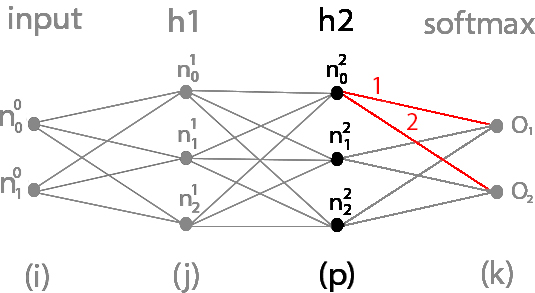
\includegraphics[scale=0.35]{imagenes/nn_h2_caminos_posibles.jpg}  
	\caption{Imagen de los 'caminos' desde la capa softmax hasta $n^2_0$}
	\label{nn_h2_caminos_posibles}
\end{figure}

Tal y como se comentó anteriormente, hay más de un 'camino' desde la capa softmax hasta $n^2_p$. Por tanto, para obtener el gradiente de la pérdida respecto a cada $n^2_p$, habría que calcular la suma de todos los ellos. \\

\begin{gather}
	\frac{\partial E_{total}}{\partial a^2_p} = \sum_{k=1}^K \frac{\partial E_k}{\partial a^2_p} = \sum_{k=1}^K  gradiente\_Z_k * \frac{\partial Z_k}{\partial z^2_p} * \frac{\partial z^2_p}{\partial a^2_p}
	\label{E_total_a2p}
\end{gather}

\begin{gather}
	\frac{\partial Z_k}{\partial z^2_p} = \frac{\partial( [\sum_{c=1}^{P} z^2_c * W^2_{ck}] + b^3_k)}{\partial z^2_p} = W^2_{pk}
	\label{deriv_Zk_z2p}
\end{gather}

\begin{figure}[H]
	\centering
	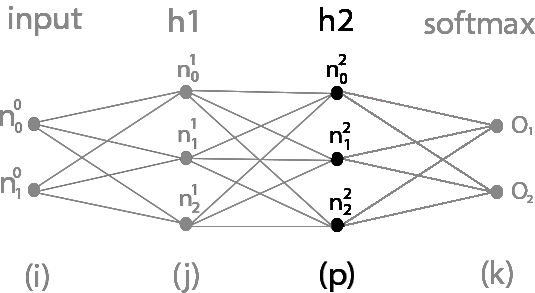
\includegraphics[scale=0.35]{imagenes/nn_2_capa_h2.jpg}  
	\caption{Imagen de backpropagation en la capa oculta h2}
	\label{fig:nn_2_capa_h2}
\end{figure}

En la capa oculta h2 se emplea la función de activación sigmoide. 

\begin{gather}
	sigmoide(x) = \frac{1}{1+e^{-x}} \\
	sigmoide'(x) = \frac{sigmoide(x)}{1-sigmoide(x)}
\end{gather}

De esta forma,


\begin{gather}
	\frac{\partial z^2_ p}{\partial a^2_p} = \frac{\partial sigmoide(a^2_p)}{\partial a^2_p} = sigmoide(a^2_p)*(1-sigmoide(a^2_p))
	\label{deriv_z2p_a2p}
\end{gather}

Se retoma la fórmula \ref{E_total_a2p} mediante la aplicación de \ref{deriv_Zk_z2p} y \ref{deriv_z2p_a2p}.

\begin{gather}
	\frac{\partial E_{total}}{\partial a^2_p} = \sum_{k=1}^K  gradiente\_Z_k * W^2_{pk} * sigmoide(a^2_p)*(1-sigmoide(a^2_p)) \\
	\frac{\partial E_{total}}{\partial a^2_p} = gradiente\_h2_p
	\label{grad_E_a2p}
\end{gather}

Una vez más, la fórmula obtenida (\ref{grad_E_a2p}) coindice con la calculada previamente (\ref{grad_E_a1p}). \\

\subsubsection{Pesos capas h1-h2}

\begin{figure}[H]
	\centering
	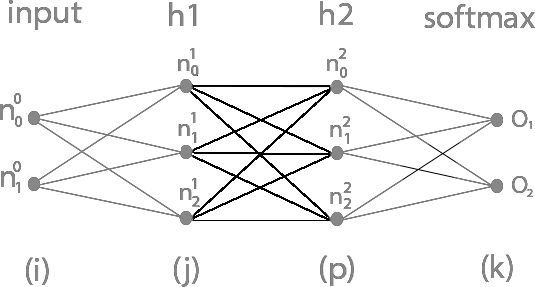
\includegraphics[scale=0.35]{imagenes/nn_2_capa_pesos_h1_h2.jpg}  
	\caption{Imagen de backpropagation en los pesos entre las capas ocultas h1 y h2}
	\label{fig:nn_2_pesos_h1_h2}
\end{figure}


\begin{gather}
	\frac{\partial a^2_p }{\partial W^1_{jp} } = \frac{\partial [\sum_{c=1}^{J} z^1_c * W^1_{cp}] + b^2_p)}{\partial W^1_{jp} } = z^1_j \\
	\frac{\partial E}{\partial W^1_{jp}} = \frac{\partial E_{total} }{\partial a^2_p } * \frac{\partial a^2_p}{W^1_{jp}} \\
	\frac{\partial E(x) }{\partial W^1_{jp} } = gradiente\_h2_p * \frac{\partial a^2_p }{\partial W^1_{jp} } = gradiente\_h2_p * z^1_j 
	\label{grad_w1jp}
\end{gather}

La fórmula \ref{grad_w1jp} vuelve a coincidir con \ref{grad_w0ip}


\subsubsection{Sesgos capa h2}

\begin{gather}
	\frac{\partial E}{\partial b^2_p} = \frac{\partial E_{total} }{\partial a^2_p } * \frac{\partial a^2_p}{b^2_p} \\
	\frac{\partial a^2_p }{\partial b^2_p } = \frac{\partial ([\sum_{c=1}^{J} z^1_c * W^1_{jp}] + b^2_p) }{\partial b^2_p } = 1 \\
	\frac{\partial E}{\partial b^2_p} = gradiente\_h2_p
	\label{grad_b2p}
\end{gather}

La fórmula \ref{grad_b2p} coincide con \ref{grad_b1p}. \\

\subsubsection{Capa oculta h1}

\begin{figure}[H]
	\centering
	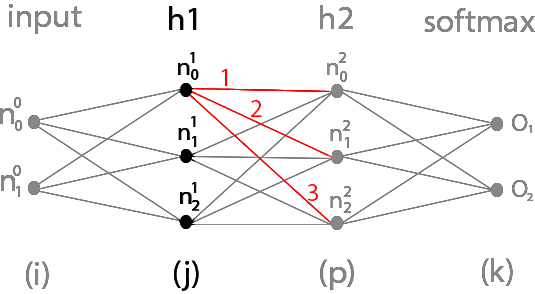
\includegraphics[scale=0.35]{imagenes/nn_h1_caminos_posibles.jpg}  
	\caption{Imagen de los 'caminos' desde la capa softmax hasta $n^1_0$}
	\label{nn_h1_caminos_posibles}
\end{figure}

De igual forma que se realizó en la capa h2, se calcula la suma de todos los 'caminos' hacia cada neurona $n^1_j$. \\

\begin{gather}
	\frac{\partial E_{total}}{\partial a^1_j} = \sum_{k=1}^K \frac{\partial E_k}{\partial a^1_j} = \sum_{p=1}^P  gradiente\_h2_p * \frac{\partial a^2_p}{\partial z^1_j} * \frac{\partial z^1_j}{\partial a^1_j} \\
	\frac{\partial a^2_p}{\partial z^1_j} = \frac{\partial( [\sum_{c=1}^{J} z^1_c * W^1_{cp}] + b^2_p)}{\partial z^1_j} = W^1_{jp}
\end{gather}

\begin{figure}[H]
	\centering
	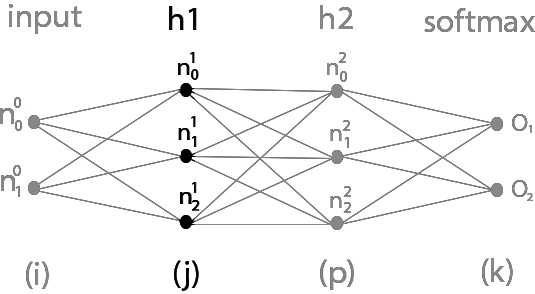
\includegraphics[scale=0.35]{imagenes/nn_2_capa_h1.jpg}  
	\caption{Imagen de backpropagation en la capa oculta h1}
\end{figure}

En la capa oculta h1 se emplea la función de activación ReLU. 

\begin{gather}
	ReLU(x) = max(0, x) \\
	ReLU'(x) = 1\ si\ x>0,\ 0\ en\ caso\ contrario
\end{gather}

De esta forma,


\begin{gather}
	\frac{\partial z^1_ j}{\partial a^1_j} = 1\ si\ x>0,\ 0\ en\ caso\ contrario \\
	\frac{\partial E_{total}}{\partial a^1_j} = \sum_{p=1}^P  gradiente\_h2_p * W^1_{jp} * ReLU'(a^1_j) \\
	\frac{\partial E_{total}}{\partial a^1_j} = gradiente\_h1_j
	\label{grad_E_a1j}
\end{gather}

El cálculo para obtener la fórmula \ref{grad_E_a1j} es muy parecido al realizado para \ref{grad_E_a2p}, pero es ``nuevo'' respecto a la sección anterior, pues esta capa no existe en dicho caso. \\


\subsubsection{Pesos capa input-h1}

\begin{figure}[H]
	\centering
	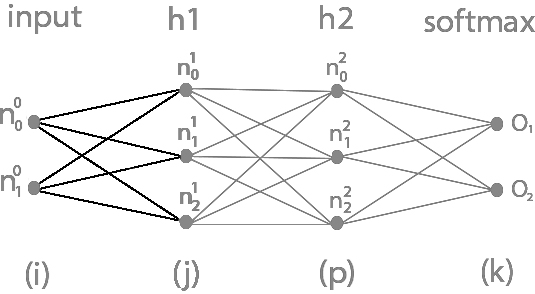
\includegraphics[scale=0.35]{imagenes/nn_2_capa_pesos_input_h1.jpg}  
	\caption{Imagen de backpropagation en los pesos entre la capa input y la capa oculta h1}
	\label{fig:nn_2_pesos_input_h1}
\end{figure}


\begin{gather}
	\frac{\partial a^1_j }{\partial W^0_{ij} } = \frac{\partial ([\sum_{c=1}^{I} z^0_c * W^0_{cj}] + b^1_j)}{\partial W^0_{ij} } = z^0_i \\
	\frac{\partial E}{\partial W^0_{ij}} = \frac{\partial E_{total} }{\partial a^1_j } * \frac{\partial a^1_j}{W^0_{ij}} \\
	\frac{\partial E(x) }{\partial W^0_{ij} } = gradiente\_h1_j * \frac{\partial a^1_j }{\partial W^0_{ij} } = gradiente\_h1_j * z^0_i 
\end{gather}

\subsubsection{Sesgos capa h1}

\begin{gather}
	\frac{\partial E}{\partial b^1_j} = \frac{\partial E_{total} }{\partial a^1_j } * \frac{\partial a^1_j}{b^1_j} \\
	\frac{\partial a^1_j }{\partial b^1_j } = \frac{\partial ([\sum_{c=1}^{I} z^0_c * W^0_{ij}] + b^1_j) }{\partial b^1_j } = 1 \\
	\frac{\partial E}{\partial b^1_j} = gradiente\_h1_j
	\label{grad_b1j}
\end{gather}

La fórmula \ref{grad_b1j} coincide con \ref{grad_b1p}. \\

\subsubsection{Capa input}

\begin{figure}[H]
	\centering
	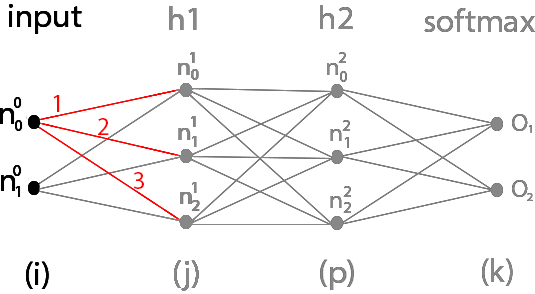
\includegraphics[scale=0.35]{imagenes/nn_2_capas_caminos_posibles_input.jpg}  
	\caption{Imagen de los 'caminos' desde la capa oculta h1 hasta $n^0_0$}
	\label{nn_2_capas_caminos_posibles_input}
\end{figure}

\begin{gather}
	\frac{\partial E_{total}}{\partial a^0_i} = \sum_{j=1}^J \frac{\partial E_{total}}{\partial a^1_j} * \frac{\partial a^1_j}{\partial z^0_i} * \frac{\partial z^0_i}{\partial a^0_i} \\
	\frac{\partial a^1_j }{\partial z^0_i } = \frac{\partial ([\sum_{c=1}^{I} z^0_c * W^0_{ij}] + b^1_j) }{\partial z^0_i } = W^0_{ij}
\end{gather}

\begin{figure}[H]
	\centering
	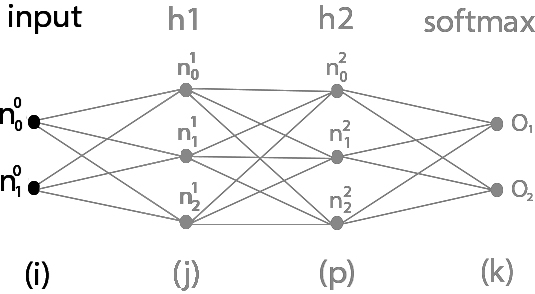
\includegraphics[scale=0.35]{imagenes/nn_2_capa_input.jpg}  
	\caption{Imagen de backpropagation en la capa input}
	\label{fig:nn_2_capa_input}
\end{figure}

Como la capa input no presenta ninguna función de activación asociada, $z^0_i$ es igual $a^0_i$. \\

\begin{gather}
	\frac{\partial z^0_i }{\partial a^0_i } = 1 \\
	\frac{\partial E_{total}}{\partial a^0_i} = \sum_{p=1}^{P} gradiente\_h1_p
\end{gather}

\subsection{Conclusiones}
Se definen como capas ocultas ``intermedias'' todas menos la última de ellas. Tal y como se ha mostrado anteriormente, comparten la mayoría del cálculo en cuanto a retropopagación. De esta forma, se puede dividir una red neuronal totalmente conectada en 4 grupos $\{$capa input, capas ocultas intermedias, última capa oculta, capa de salida o capa softmax$\}$. \\
A continuación se realiza el cálculo necesario para la retropropagación de una capa de neuronas l determinada. Suponemos que la capa l+1 tiene Q neuronas, la capa l-1 tiene K neuronas, y todas las capas ocultas intermedias usan ReLU como función de activación. \\

\subsubsection{Gradiente respecto a la entrada}

\begin{figure}[H]
	\centering
	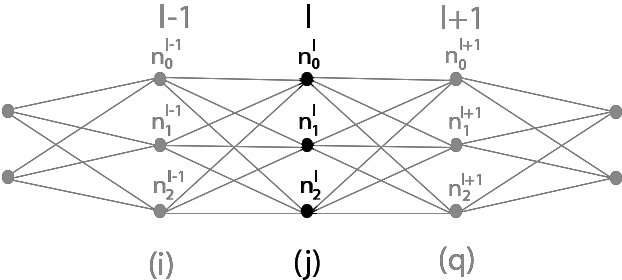
\includegraphics[scale=0.35]{imagenes/conclusion_capa_l.jpg}  
	\caption{Imagen de backpropagation en la capa l}
	\label{fig:conclusion_capa_l}
\end{figure}

\begin{gather}
	\frac{\partial E_{total}}{\partial a^l_j} = \sum_{q=1}^Q \frac{\partial E_{total}}{\partial a^{l+1}_q} * \frac{\partial a^{l+1}_q}{\partial z^l_j} * \frac{\partial z^l_j}{\partial a^l_j} \\
	\frac{\partial a^{l+1}_j }{\partial z^l_j } = \frac{\partial ([\sum_{c=1}^{K} z^l_c * W^l_{ij}] + b^{l+1}_j) }{\partial z^l_j } = W^l_{ij} \\
	\frac{\partial z^l_j}{\partial a^l_j} = ReLU'(a^l_j) \\
	\frac{\partial E_{total}}{\partial a^l_j} = \sum_{q=1}^Q  gradiente\_h_{{l+1}_q} * W^l_{ij} * ReLU'(a^l_j) \\
	\frac{\partial E_{total}}{\partial a^l_j} = gradiente\_h_{l_j}
\end{gather}

\subsubsection{Gradiente respecto a los pesos}

\begin{figure}[H]
	\centering
	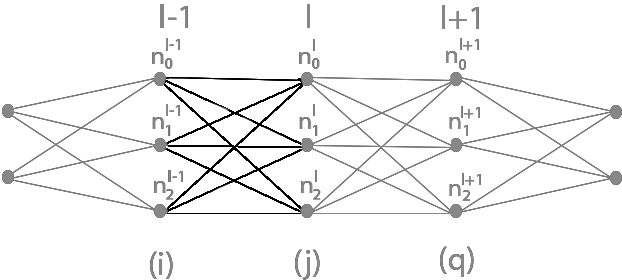
\includegraphics[scale=0.35]{imagenes/conclusion_pesos.jpg}  
	\caption{Imagen de backpropagation en los pesos entre la capa l-1 y l}
	\label{fig:conclusion_pesos}
\end{figure}

\begin{gather}
	\frac{\partial E}{\partial W^{l-1}_{ij}} = \frac{\partial E_{total} }{\partial a^l_j } * \frac{\partial a^l_j}{W^{l-1}_{ij}} \\
	\frac{\partial a^l_j }{\partial W^{l-1}_{ij} } = \frac{\partial ([\sum_{c=1}^{K} z^{l-1}_c * W^{l-1}_{cj}] + b^l_j)}{\partial W^{l-1}_{ij} } = z^{l-1}_i \\
	\frac{\partial E(x) }{\partial W^{l-1}_{ij} } = gradiente\_h_{l_j} * \frac{\partial a^l_j }{\partial W^{l-1}_{ij} } = gradiente\_h_{l_j} * z^{l-1}_i 
\end{gather}

\subsubsection{Gradiente respecto a sesgos}

\begin{gather}
	\frac{\partial E}{\partial b^l_j} = \frac{\partial E_{total} }{\partial a^l_j } * \frac{\partial a^l_j}{b^l_j} \\
	\frac{\partial a^l_j }{\partial b^l_j } = \frac{\partial ([\sum_{c=1}^{K} z^{l-1}_c * W^{l-1}_{ij}] + b^l_j) }{\partial b^l_j } = 1 \\
	\frac{\partial E}{\partial b^l_j} = gradiente\_h_{l_j}
\end{gather}

\section{Paralelización en entrenamiento}

\subsubsection{Tipos de paralelismo}

El entrenamiento de una red neuronal convolucional (CNN) se puede paralelizar de distintas formas. Si el modelo se reparte entre varios ordenadores que son entrenados con los mismos datos, se denomina \textbf{paralelismo del modelo} (una capa por computador, por ejemplo). Sin embargo, si se distribuyen los datos entre múltiples nodos pero se emplea el mismo modelo para entrenar, se denomina \textbf{paralelismo de datos}. \\

\subsubsection{Paralelismo en SGD}
Dada la naturaleza iterativa del algoritmo del descenso del gradiente estocástico, puede parecer un obstáculo ante la paralelización del entrenamiento del modelo. Sin embargo, tal y como se indica en \cite{CNN_parallel_Stanford}, \cite{CNN_parallel_International_Conference}, y \cite{CNN_parallel_Ome_Weird_Trick}, esto no tiene por qué ser así, pues en cada iteración se entrena al modelo con M subconjuntos de datos disjuntos entre ellos. Esto permite aplicar una paralelización de datos, de forma que cada subconjunto de M se procese en paralelo con el resto pero sobre el mismo modelo. \\
Además, \cite{CNN_parallel_International_Conference} propone un nuevo enfoque caracterizado por el aprovechamiento del tiempo de comunicación mediante cómputo en paralelo. \\

\subsubsection{Aprovechamiento del tiempo de comunicación}
En la propagación hacia detrás, se calcula el gradiente de la función de error respecto a cada parámetro de la red. Como no hay dependencia de datos entre los gradientes de distintas capas, la comunicación para intercambiar dichos gradientes entre los nodos de cálculo puede ejecutarse de manera concurrente con los cálculos de otras capas.
